\documentclass{article}
\usepackage[utf8]{inputenc}
\usepackage{geometry}
\usepackage{booktabs}
\usepackage{pgfplots}
\usepackage{times} 
\usepackage{xurl}
\usepackage{longtable}
\usepackage{url}
\usepackage{listings}
\usepackage{listings}
\usepackage{xcolor}

\definecolor{codegreen}{rgb}{0,0.6,0}
\definecolor{codegray}{rgb}{0.5,0.5,0.5}
\definecolor{codepurple}{rgb}{0.58,0,0.82}
\definecolor{codeblue}{rgb}{0.5,0.9,0.9}

\lstdefinestyle{mystyle}{
  commentstyle=\large\color{codeblue},
  keywordstyle=\large\color{codegreen},
  numberstyle=\large\color{codegray},
  stringstyle=\large\color{codepurple},
  basicstyle=\ttfamily\footnotesize\large,
  breakatwhitespace=false,         
  breaklines=true,                 
  captionpos=b,                    
  keepspaces=true,                 
  numbers=left,                    
  numbersep=12pt,                  
  showspaces=false,                
  showstringspaces=false,
  showtabs=false,                  
  tabsize=2
}

\lstset{style=mystyle}
\geometry{left=2cm,right=2cm,top=2cm,bottom=2cm}
\usepgfplotslibrary{external}
\tikzexternalize

\begin{document}
\large
\begin{titlepage}
\begin{figure}[t]
    \centering\includegraphics[width=0.3\textwidth]{img/School.png}
\end{figure}
\begin{center}
    \textsc{ \LARGE{Mathematics Project Competition for Secondary Schools(2021/22)\\}}
	\textsc{ \LARGE{Category A(Junior secondary project)\\ }}
	\textnormal{ \LARGE{Sha Tin Government Secondary School\\}}
	\vspace{30mm}
	\fontsize{10mm}{7mm}\selectfont 
    \textup{The COVID testing problem}\\
\end{center}

\vspace{25mm}

\begin{minipage}[t]{0.47\textwidth}
	\textnormal{\large{\bf Teacher Supervisor:\\}}
	{\large KN\\CSA\\TCK}
\end{minipage}\hfill\begin{minipage}[t]{0.47\textwidth}\raggedleft
	\textnormal{\large{\bf Candidates:\\}}
	{\large 3D 01 He Huang Zhen\\3D 04 Lam Kwan Ho\\3D 06 Leung Ka Hei\\3D 15 Cheng Man Hei\\3D 27 Li Lok Yin\\3D 31 Wong Ka Fun}
\end{minipage}

\vspace{20mm}

\centering{\large{Finish date:22/02/2022}}

\end{titlepage}
\tableofcontents
\newpage
\section{Introduction}
\subsection{Introduction}
During the pandemic of COVID-19(SARS-CoV-2), the demand for virus testing dramatically increases, so as the cost and wastes caused during the tests. By the traditional way, the subject is tested one by one, meaning that the amount of test conducted is as same as the number of subjects. When a huge amount of population need to be tested, overloading in laboratories will be leaded and a huge amount of waste will be generated. In this paper, we are going to investigate how to increase the efficiency of conducting test with less amount of test by pooling the samples together and doing multiple tests. We want to find a better solution for different conditions.
\subsection{Problem restatement}
\begin{enumerate}
  \item Develop a mathematical model for determining the most efficient testing method of COVID-19 for a large population. Discuss the factors taken into consideration, use the model to chose the most efficient way for testing (i.e. lower the total tests required).
  \item Finding the most efficient way of pooling test when the sample is grouped once
    \begin{enumerate}
     \item Choose an example from one of the cites around the Earth, and develop a mathematical model(or models) from any factors and data obtainable and we find significant for determining the optimum solution for the situation. Analyzing the result.
     \item Discuss any changes to the COVID-19 test model from that would be required to determine the result of the model.
    \end{enumerate}
  \item Discuss any changes to the COVID-19 test model that will be required when we consider regrouping.
  \item Compare different groupings effectiveness by the result.
\end{enumerate}
\section{Definition and Assumptions}

\subsection{Definition of important terms in the paper}
\begin{tabular}{p{5cm}p{12cm}}
\toprule
\textbf{Terms in the paper}&\textbf{Definition}\\
\toprule
COVID-19&Coronavirus disease 2019 (COVID-19) is the disease caused by a new coronavirus called SARS-CoV-2. The most common symptoms of COVID-19 include fever, dry cough and fatigue.\cite{covid19def}\\
\midrule
Pandemic&(of a disease) existing in almost all of an area or in almost all of a group of people, animals, or plants\cite{pandemicdef}\\
\midrule
Tests&Test for determining the virus's occurrence in the subject, including Deep Throat Saliva Test, Combined Nasal and Throat Swabs Test, Nasopharyngeal swab Test, and Antibody Test.\cite{testsdef}\\
\midrule
Pooling test&Mixing samples together before testing and test the mixed sample in order to use less test resources\cite{pooldef}\\
\bottomrule
\end{tabular}

\subsection{Definition of Variables}
\begin{tabular}{p{5cm}p{12cm}}
\toprule
\textbf{Variable}&\textbf{Definition}\\
\toprule
$N$&Total number of population to be tested\\
\midrule
$n$&The group size\\
\midrule
$p$&The infection rate of COVID-19 in a certain population\\
\bottomrule
\end{tabular}

\subsection{General Assumptions and Justifications}
\begin{tabular}{p{8.5cm}p{8.5cm}}
\toprule
\textbf{Assumption}&\textbf{Justification}\\
\toprule
The test result is 100\% accurate and there will never be a false positive or false negative result in the test&This is for the ease of the construction of the model\\
\midrule
There isn't a limit for the amount of samples tested once&This is for the ease of the construction of the model\\
\midrule
The amount of samples collected at once is enough for doing the test required&This is for the ease of the construction of the model\\
\bottomrule
\end{tabular}
\section{Simple model}
We start with the simplest form of this problem. With a fixed number of people waiting to be tested, when does it take fewer total tests if the samples are pooled and tested together first. Since $p$ is the infection rate , the probability of not infected will be $(1-p)$.
\subsection{Two samples}
For testing 2 samples in ideal solution, we consider the following possibilities:

\begin{itemize}
  \item For all the samples negative. The probability is $(1-p)^2$. Only 1 test is required.
  \item For 1 of the samples positive, 1 of the samples negative. The probability is $p(1-p)$. 3 tests is required. But if the first sample is tested negative, only 2 test is required as the last sample must be positive.
  \item For all the samples positive. The probability is $p^2$. 3 tests is required.
\end{itemize}
Similarly, the expected number of test:
\\
\begin{displaymath}
t(p)=3p^2+(1-p)^2+2(1-p)p+3p(1-p)
\end{displaymath}
\\
Simplifying $t(p)$, we get:
\\
\begin{displaymath}
t(p)=-p^2+3p+1
\end{displaymath}
\\
For solving $t(p)=2$, we get:
\\
\begin{center}
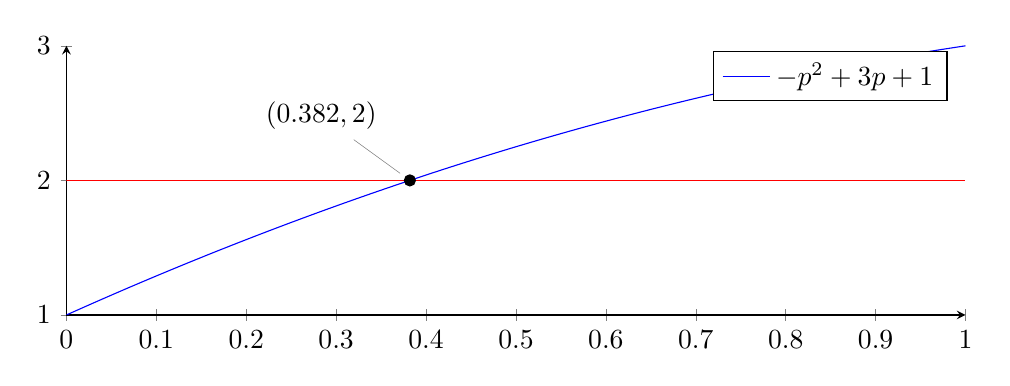
\begin{tikzpicture}
\begin{axis}[
    axis lines = left,
    ytick={0,1,2,3},
    xtick={0,0.1,0.2,0.3,0.4,0.5,0.6,0.7,0.8,0.9,1},
    height=5cm,
    width=13cm,
]

\addplot [
    domain=0:1, 
    samples=1000, 
    color=blue,
    ]
    {-x^2 + 3*x + 1};
\addlegendentry{\(-p^2+3p+1\)}

\addplot [
    domain=0:1, 
    samples=100, 
    color=red,
    ]
    {2};
    
\addplot[mark=*] coordinates {(0.382,2)} node[pin=120:{$(0.382,2)$}]{} ;

\end{axis}
\end{tikzpicture}
\end{center}
\\
From the graph, we find that when the group size is equal to 2, pooling should be used only when $p<0.382$ such that the expected amount of tests used is lower than the traditional way.

\subsection*{Worse Case of Two Samples}
If the first grouping test is positive, the samples had to be retested individually. From the method above, we considered a special case of testing: If all of the samples tested before the last one got a negative result, we assume that the last sample must be positive. But in reality, the samples may not be tested one by one but simultaneously. Which means that this special case may not exist in reality, for example, in a sample of 2, for 1 of the samples positive, 1 of the samples negative.  The probability is $p(1 -− p)$. The case for only 2 test is required as the last sample must be positive will not be considered, such that there will only be neither 1 test or 3 tests used in every group.
\\
\\
Similar to the ideal 2 sample test, we consider the following possibilities:

\begin{itemize}
  \item For all the samples negative. The probability is $(1-p)^2$. Only 1 test is required.
  \item For 1 of the samples positive, 1 of the samples negative. The probability is $p(1-p)$. 3 tests is required. 
  \item For all the samples positive. The probability is $p^2$. 2 tests is required.
\end{itemize}
The new expected number of test will be given out by:
\\
\begin{displaymath}
T(p)=3p^2 + 3p(1-p) \times 2 + 1(1-p)^2
\end{displaymath}
\\
Simplifying $T(p)$, we get:
\\
\begin{displaymath}
T(p)=-2p^2+4p+1
\end{displaymath}
\\
For solving $T(p)=2$, we get:
\\
\begin{center}
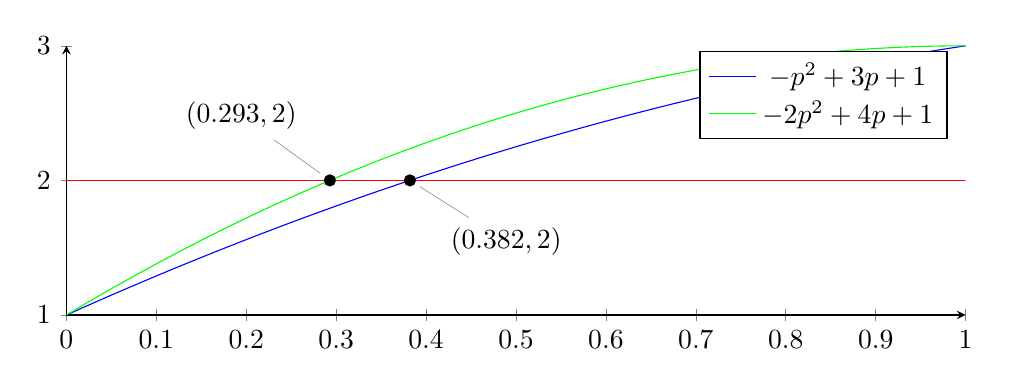
\begin{tikzpicture}
\begin{axis}[
    axis lines = left,
    ytick={0,1,2,3},
    xtick={0,0.1,0.2,0.3,0.4,0.5,0.6,0.7,0.8,0.9,1},
    height=5cm,
    width=13cm,
]

%Here the blue parabola is defined
\addplot [
    domain=-0:1, 
    samples=100, 
    color=blue,
    ]
    {-x^2 + 3*x + 1};
\addlegendentry{\(-p^2+3p+1\)}

%Here the red parabola is defined
\addplot [
    domain=0:1, 
    samples=100, 
    color=green,
    ]
    {-2*x^2 + 4*x + 1};
\addlegendentry{\(-2p^2+4p+1\)}

%Here y=2 is defined
\addplot [
    domain=0:1, 
    samples=100, 
    color=red,
    ]
    {2};

%Two dots are defined
\addplot[mark=*] coordinates {(0.293,2)} node[pin=120:{$(0.293,2)$}]{} ;
\addplot[mark=*] coordinates {(0.382,2)} node[pin=310:{$(0.382,2)$}]{} ;

\end{axis}
\end{tikzpicture}
\end{center}
\\
From the graph, we find that in the worse case, when the group size is equal to 2, pooling should be used only when $p<0.293$ such that the expected amount of tests used is lower than the traditional way.
\\
\\
We can compare the two expected functions by considering the difference:
\\
\begin{displaymath}
D(p)=T(p)-t(p)=-2p^2+4p+1-(-p^2+3p+1)
\end{displaymath}
\\
Solving $D(p):$
\\
\begin{displaymath}
D(p)=-p^2+p
\end{displaymath}
\\
The difference of the two equations is a cubic equation.
\\
\\
Graphing the equation:
\\
\begin{center}
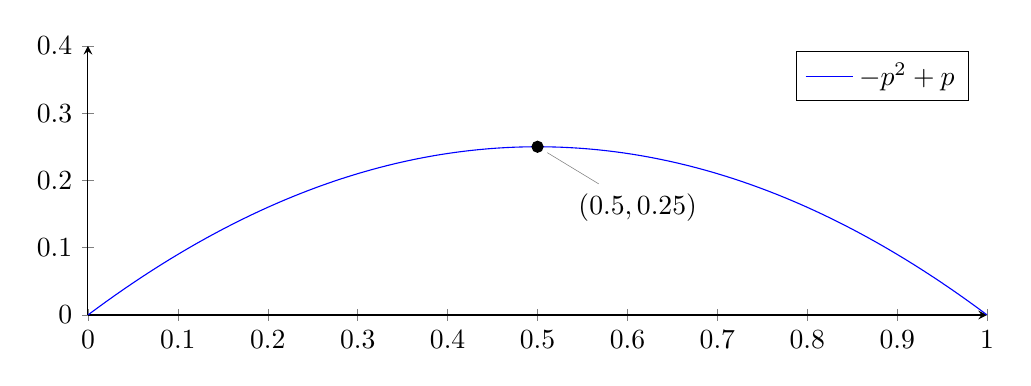
\begin{tikzpicture}
\begin{axis}[
    axis lines = left,
    ytick={0,0.1,0.2,0.3,0.4},
    ymin=0.0,ymax=0.4,
    xtick={0,0.1,0.2,0.3,0.4,0.5,0.6,0.7,0.8,0.9,1},
    height=5cm,
    width=13cm,
]

%Here the blue parabola is defined
\addplot [
    domain=0:1, 
    samples=100, 
    color=blue,
    ]
    {-x^2 +x};
\addlegendentry{\(-p^2+p\)}

%Two dots are defined
\addplot[mark=*] coordinates {(0.5,0.25)} node[pin=310:{$(0.5,0.25)$}]{} ;

\end{axis}
\end{tikzpicture}
\end{center}
\\
From the graph, we noticed that the vertex of the equation is $(0.5,0.25)$, which means that the biggest difference occurs when $p=0.5$ and the expected value of the two models differ by 0.25 tests.
\subsection{Three samples}
For testing 3 samples in ideal solution, we consider the following possibilities:

\begin{itemize}
  \item For all the samples negative. The probability is $(1-p)^3$. Only 1 test is required.
  \item For 1 of the samples positive, 2 of the samples negative. The probability is $p(1-p)^2$. 4 tests is required. But if the first 2 samples are tested negative, only 3 test is required as the last sample must be positive.
  \item For all the samples positive. The probability is $p^3$. 4 tests is required.
  \item For 2 of the samples positive, 1 negative. The probability is $p^2(1-p)$.  4 tests is required.
\end{itemize}
The expected number of test:
\\
\begin{displaymath}
t(p)=4p^{3}+1(1-p)^{3}+4p^{2}(1-p) \times 3+4p(1-p)^{2} \times 2+3p(1-p)^{2}
\end{displaymath}
\\
Simplifying $t(p)$, we get:
\\
\begin{displaymath}
t(p)=2p^{3}-7p^{2}+8p+1
\end{displaymath}
\\
For solving $t(p)=3$:

\begin{center}
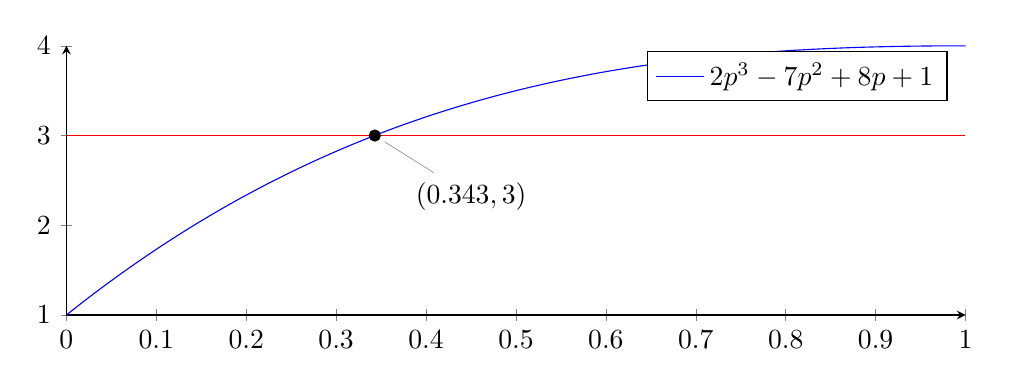
\begin{tikzpicture}
\begin{axis}[
    axis lines = left,
    ytick={0,1,2,3,4},
    xtick={0,0.1,0.2,0.3,0.4,0.5,0.6,0.7,0.8,0.9,1},
    height=5cm,
    width=13cm,
]

\addplot [
    domain=0:1, 
    samples=1000, 
    color=blue,
    ]
    {2*x^3 - 7*x^2 + 8*x + 1};
\addlegendentry{\(2p^{3}-7p^{2}+8p+1\)}

\addplot [
    domain=0:1, 
    samples=100, 
    color=red,
    ]
    {3};
    
\addplot[mark=*] coordinates {(0.343,3)} node[pin=310:{$(0.343,3)$}]{} ;

\end{axis}
\end{tikzpicture}
\end{center}
\\
From the graph, we find that when the group size is equal to 3, pooling should be used only when $p<0.343$ such that the expected amount of tests used is lower than the traditional way.

\subsection*{Worse Case of Three Samples}
\\
\\
Similar to the ideal 3 sample test, we consider the following possibilities:

\begin{itemize}
  \item For all the samples negative. The probability is $(1-p)^3$. Only 1 test is required.
  \item For 1 of the samples positive, 2 of the samples negative. The probability is $p(1-p)^2$. 4 tests is required.
  \item For all the samples positive. The probability is $p^3$. 4 tests is required.
  \item For 2 of the samples positive, 1 negative. The probability is $p^2(1-p)$.  4 tests is required.
\end{itemize}
The new expected number of test will be given out by:
\\
\begin{displaymath}
T(p)=4p^{3}+4p^{2}(1-p) \times 3+4p(1-p)^{2} \times 3 +1(1-p)^{3}
\end{displaymath}
\\
Simplifying $T(p)$, we get:
\\
\begin{displaymath}
T(p)=3p^3-9p^2+9p+1
\end{displaymath}
\\
For solving $T(p)=3$, we get:
\\
\begin{center}
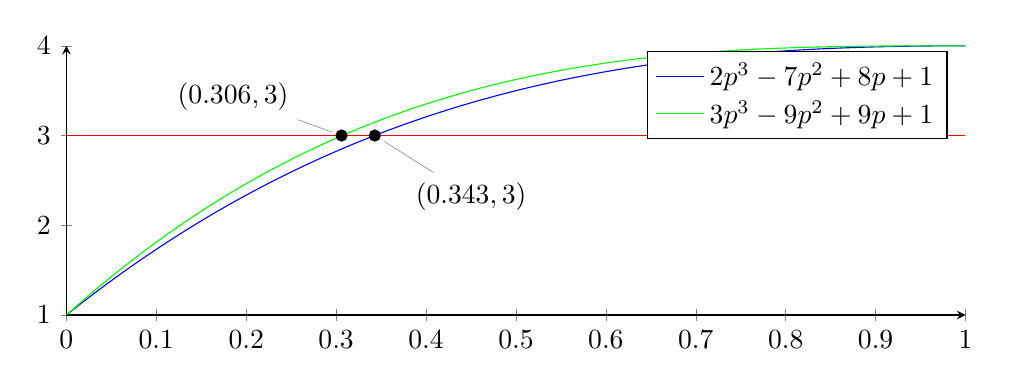
\begin{tikzpicture}
\begin{axis}[
    axis lines = left,
    ytick={1,2,3,4,5},
    xtick={0,0.1,0.2,0.3,0.4,0.5,0.6,0.7,0.8,0.9,1},
    height=5cm,
    width=13cm,
]

\addplot [
    domain=0:1, 
    samples=1000, 
    color=blue,
    ]
    {2*x^3 - 7*x^2 + 8*x + 1};
\addlegendentry{\(2p^{3}-7p^{2}+8p+1\)}

\addplot [
    domain=-0:1, 
    samples=100, 
    color=green,
    ]
    {3*x^3 - 9*x^2 + 9*x + 1};
\addlegendentry{\(3p^3-9p^2+9p+1\)}

\addplot [
    domain=0:1, 
    samples=100, 
    color=red,
    ]
    {3};

\addplot[mark=*] coordinates {(0.306,3)} node[pin=160:{$(0.306,3)$}]{} ;
\addplot[mark=*] coordinates {(0.343,3)} node[pin=310:{$(0.343,3)$}]{} ;

\end{axis}
\end{tikzpicture}
\end{center}
\\
From the graph, we find that in the worse case, when the group size is equal to 3, pooling should be used only when $p<0.306$ such that the expected amount of tests used is lower than the traditional way.
\\
\\
We can compare the two expected functions by considering the difference:
\\
\begin{displaymath}
D(p)=T(p)-t(p)=3p^3-9p^2+9p+1-(2p^{3}-7p^{2}+8p+1)
\end{displaymath}
\\
Solving $D(p):$
\\
\begin{displaymath}
D(p)=-p^2+p
\end{displaymath}
\\
The difference of the two equations is a quadratic equation.
\\
\\
Graphing the equation:
\\
\begin{center}
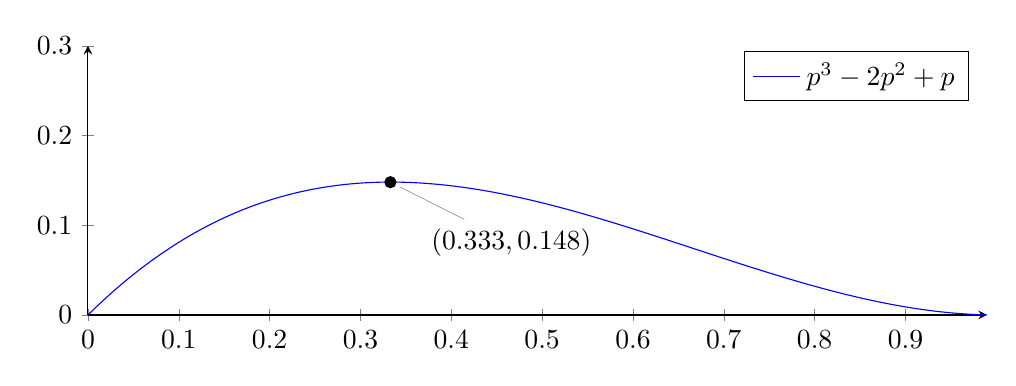
\begin{tikzpicture}
\begin{axis}[
    axis lines = left,
    ytick={0,0.1,0.2,0.3},
    ymin=0.0,ymax=0.3,
    xtick={0,0.1,0.2,0.3,0.4,0.5,0.6,0.7,0.8,0.9,1},
    height=5cm,
    width=13cm,
]

%Here the blue parabola is defined
\addplot [
    domain=0:1, 
    samples=100, 
    color=blue,
    ]
    {x^3 -2*x^2 +x};
\addlegendentry{\(p^3 -2p^2+p\)}

%Two dots are defined
\addplot[mark=*] coordinates {(0.333,0.148)} node[pin=310:{$(0.333,0.148)$}]{} ;

\end{axis}
\end{tikzpicture}
\end{center}
\\
From the graph, we can see that the vertex of the equation is $(0.333,0.148)$, which means that the biggest difference occurs when $p=0.333$ and the expected value of the two models differ by 0.148 tests.
\subsection{Four samples}
For testing 4 samples in ideal solution, we consider the following possibilities:

\begin{itemize}
  \item For all the samples negative. The probability is $(1-p)^4$. Only 1 test is required.
  \item For 1 of the samples positive, 3 of the samples negative. The probability is $p(1-p)^3$. 5 tests is required. But if the first three samples are tested negative, only 4 test is required as the last sample must be positive.
  \item For all the samples positive. The probability is $p^4$. 5 tests is required.
  \item For 3 of the samples positive and 1 negative. The probability is $p^3(1-p)$.  5 tests is required.
  \item For 2 of the samples positive, 2 negative. The probability is $p^2(1-p)^2$.  5 tests is required.
  \item For all the samples positive. The probability is $(1-p)^4$. 5 tests is required. 
\end{itemize}
Similarly, the expected number of test:
\\
\begin{displaymath}
Q(p)=5p^{4}+5p^{3}(1-p) \times 4+5 p^{2}(1-p)^{2} \times 6+5p(1-p)^{3} \times 3+4p(1-p)^{3}+1(1-p)^{4}
\end{displaymath}
\\
Simplifying $Q(p)$, we get:
\\
\begin{displaymath}
Q(p)=-3p^{4}+13p^{3}-21p^{2}+15p+1
\end{displaymath}
\\
For solving $Q(p)=4$:
\begin{center}
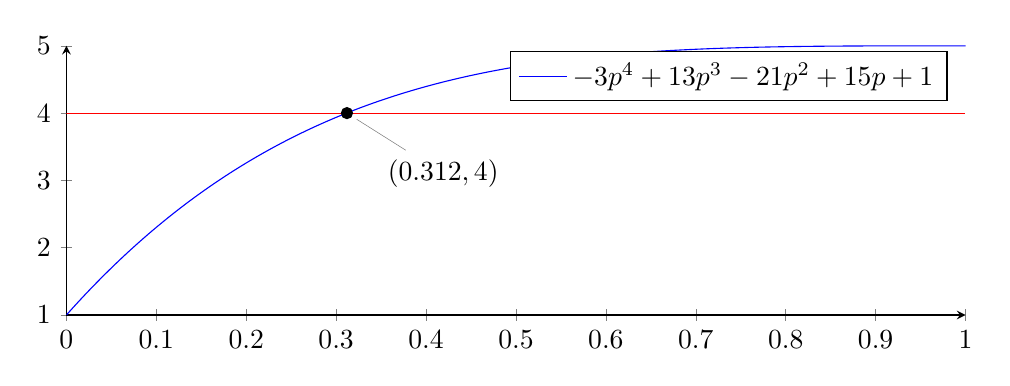
\begin{tikzpicture}
\begin{axis}[
    axis lines = left,
    ytick={1,2,3,4,5},
    xtick={0,0.1,0.2,0.3,0.4,0.5,0.6,0.7,0.8,0.9,1},
    height=5cm,
    width=13cm
]

\addplot [
    domain=0:1, 
    samples=1000, 
    color=blue,
    ]
    {-3*x^4 + 13*x^3 - 21*x^2 + 15*x + 1};
\addlegendentry{\(-3p^{4}+13p^{3}-21p^{2}+15p+1\)}

\addplot [
    domain=0:1, 
    samples=100, 
    color=red,
    ]
    {4};
\addplot[mark=*] coordinates {(0.312,4)} node[pin=310:{$(0.312,4)$}]{} ;

\end{axis}
\end{tikzpicture}
\end{center}
\\
From the graph, we find that when the group size is equal to 4, pooling should be used only when $p<0.312$ such that the expected amount of tests used is lower than the traditional way.

\subsection*{Worse Case of Four Samples}
\\
\\
Similar to the ideal 4 sample test, we consider the following possibilities:

\begin{itemize}
  \item For all the samples negative. The probability is $(1-p)^4$. Only 1 test is required.
  \item For 1 of the samples positive, 3 of the samples negative. The probability is $p(1-p)^3$. 5 tests is required.
  \item For all the samples positive. The probability is $p^4$. 5 tests is required.
  \item For 3 of the samples positive and 1 negative. The probability is $p^3(1-p)$.  5 tests is required.
  \item For 2 of the samples positive, 2 negative. The probability is $p^2(1-p)^2$.  5 tests is required.
  \item For all the samples positive. The probability is $(1-p)^4$. 5 tests is required. 
\end{itemize}
The new expected number of test will be given out by:
\\
\begin{displaymath}
T(p)=5p^{4}+5p^{3}(1-p) \times 4+5 p^{2}(1-p)^{2} \times 6+5p(1-p)^{3} \times 4+1(1-p)^{4}
\end{displaymath}
\\
Simplifying $T(p)$, we get:
\\
\begin{displaymath}
T(p)=-4p^4+16p^3-24p^2+16p+1
\end{displaymath}
\\
For solving $T(p)=3$, we get:
\\
\begin{center}
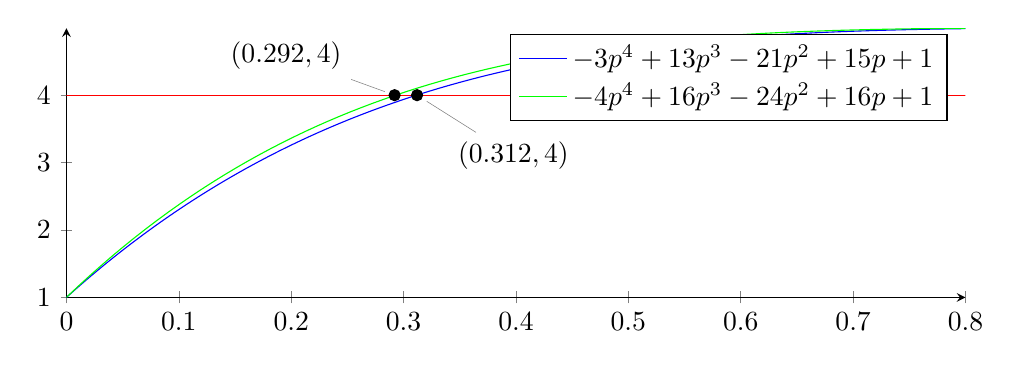
\begin{tikzpicture}
\begin{axis}[
    axis lines = left,
    ytick={1,2,3,4,5},
    xmin=0.0,xmax=0.8,
    xtick={0,0.1,0.2,0.3,0.4,0.5,0.6,0.7,0.8},
    height=5cm,
    width=13cm,
]

\addplot [
    domain=0:1, 
    samples=1000, 
    color=blue,
    ]
    {-3*x^4 + 13*x^3 - 21*x^2 + 15*x + 1};
\addlegendentry{\(-3p^{4}+13p^{3}-21p^{2}+15p+1\)}

\addplot [
    domain=-0:1, 
    samples=100, 
    color=green,
    ]
    {-4*x^4+16*x^3-24*x^2+16*x+1};
\addlegendentry{\(-4p^4+16p^3-24p^2+16p+1\)}

\addplot [
    domain=0:1, 
    samples=100, 
    color=red,
    ]
    {4};

\addplot[mark=*] coordinates {(0.292,4)} node[pin=160:{$(0.292,4)$}]{} ;
\addplot[mark=*] coordinates {(0.312,4)} node[pin=310:{$(0.312,4)$}]{} ;

\end{axis}
\end{tikzpicture}
\end{center}
\\
From the graph, we find that in the worse case, when the group size is equal to 3, pooling should be used only when $p<0.292$ such that the expected amount of tests used is lower than the traditional way. Also, we noticed that the range of  p $(p<)$ is as same as when sample equals to 2.
\\
\\
We can compare the two expected functions by considering the difference:
\\
\begin{displaymath}
D(p)=T(p)-t(p)=-4p^4+16p^3-24p^2+16p+1-(-3p^{4}+13p^{3}-21p^{2}+15p+1)
\end{displaymath}
\\
Solving $D(p):$
\\
\begin{displaymath}
D(p)=-p^4+3p^3-3p^2+p
\end{displaymath}
\\
The difference of the two equations is a quadratic equation.
\\
\\
Graphing the equation:
\\
\begin{center}
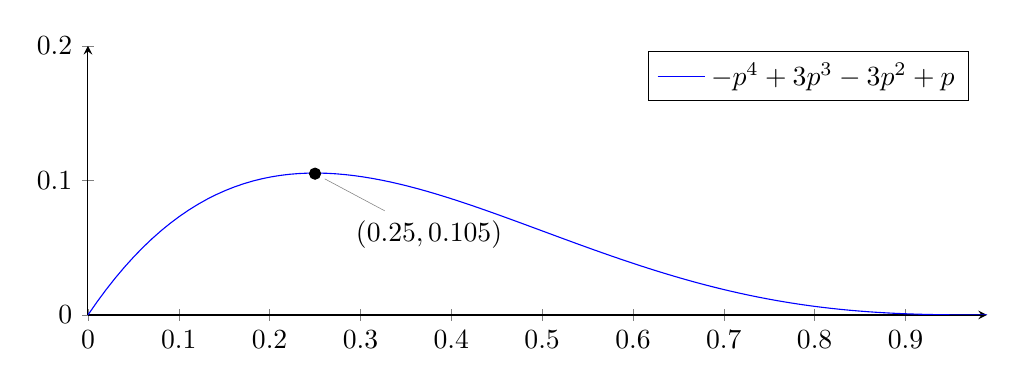
\begin{tikzpicture}
\begin{axis}[
    axis lines = left,
    ytick={0,0.1,0.2},
    ymin=0.0,ymax=0.2,
    xtick={0,0.1,0.2,0.3,0.4,0.5,0.6,0.7,0.8,0.9,1},
    height=5cm,
    width=13cm,
]

%Here the blue parabola is defined
\addplot [
    domain=0:1, 
    samples=100, 
    color=blue,
    ]
    {-x^4 + 3*x^3 -3*x^2 +x};
\addlegendentry{\(-p^4+3p^3-3p^2+p\)}

%Two dots are defined
\addplot[mark=*] coordinates {(0.25,0.105)} node[pin=310:{$(0.25,0.105)$}]{} ;

\end{axis}
\end{tikzpicture}
\end{center}
\\
From the graph, we can see that the vertex of the equation is $(0.25,0.105)$, which means that the biggest difference occurs when $p=0.25$ and the expected value of the two models differ by 0.148 tests.
\subsection{General term of the Worse Case}
As the method mentioned above, we are considering if the first grouping test is positive, the samples had to be retested individually. We did not include the special case, and in fact this make our calculation much easier. As the inflection rate is $p$ and the rate of not inflected is $(1-p)$, we know that all the combinations of the possibilities can be found with $(p+(1-p))^n$. Which is not useful then as we need to locate the special case. As we are not considering it, with less complexity, we can modify a general term to find out $T(p)$ for any group size $n$ by following steps.
\\
\\
Expanding $(p+(1-p))^n$:
\\
\\
\begin{array}{l}
(p+(1-p))^n\\
=p^{n} +C_{1}^{n}  \cdot p^{n-1} \left ( 1-p \right ) +C_{2}^{n }  \cdot p^{n-2} \left ( 1-p \right )^{2} +\dots +C_{G-1}^{n}  \cdot p^{n-\left ( n-1 \right ) } \left ( 1-p \right )^{n-1} +\left ( 1-p \right ) ^{n}\\
\end{array}
\\
\\
\\
By the General Term of Binomial Theorem, $(p+(1-p))^n$ can be expanded as above.
\\
\\
As we know that if there is at least one people inflected in the group, the number of test needed for the whole group is $(n+1)$ and if nobody was inflected in the group, only 1 test will be used. To find out T(p), we can multiply 1 to $(1-p)^n$ and multiply $(n+1)$ to all the terms remaining, such that the general term of expecting number of tests can be given out by:
\\
\\
\begin{array}{l}
T(p)=\left ( n+1 \right ) \left [ p^{n} +C_{1}^{n }  \cdot p^{n-1} \left ( 1-p \right ) +C_{2}^{n }  \cdot p^{n-2} \left ( 1-p \right )^{2} +\dots +C_{n-1}^{n }  \cdot p^{n-\left ( n-1 \right ) } \left ( 1-p \right )^{n-1} \right ]\\+\left 1( 1-p \right ) ^{n}
\end{array}
\\
\\
\\
By this general term, we don't need to count the combinations one by one like in the past, which dramatically increased the efficiency. Also, with less complexity, we can develop a program using Python and MATLAB easily to generate the equation of the expected value T(p) and find out the range of p $(p<)$ of any group size n . We also included the results when n = 2 to 100 from our calculation. \textbf{[Appendix 9.1]}

\subsection{Results}
The ideal sample results is summarized on the following table:
\\
\\
\begin{tabular}{p{5.25cm}p{5.25cm}p{6cm}}
\toprule
\textbf{Group size}&\textbf{Coordinate}&\textbf{Probability required}\\
\toprule
2&$(0.382,2)$&$p<0.382$\\
\midrule
3&$(0.343,3)$&$p<0.343$\\
\midrule
4&$(0.312,4)$&$p<0.312$\\
\bottomrule
\end{tabular}
\\
\\
\\
Observing the pattern, we found that the requirement of the infection rate $p$ increases as the groups size increases for the ideal solution.
\\
\\
The worse case results is summarized on the following table:
\\
\\
\begin{tabular}{p{5.25cm}p{5.25cm}p{6cm}}
\toprule
\textbf{Group size}&\textbf{Coordinate}&\textbf{Probability required}\\
\toprule
2&$(0.293,2)$&$p<0.293$\\
\midrule
3&$(0.306,3)$&$p<0.306$\\
\midrule
4&$(0.293,4)$&$p<0.293$\\
\bottomrule
\end{tabular}
\\
\\
\\
Observing the pattern, we found that the requirement of the infection rate $p$ is the same when sample size equal to 2 and 4 for the ideal solution. As we also calculated the range of $p$ for the worse case by program, from the data we get, we found that 3 have the highest comparability of range of $p$. Similar the ideal solution, the requirement of the infection rate $p$ increases as the groups size increases for the ideal solution after 4.\textbf{[Appendix 9.1]}
\\
\\
The difference results is summarized on the following table:
\\
\\
\begin{tabular}{p{3cm}p{3.5cm}p{3.5cm}p{6cm}}
\toprule
\textbf{Group size}&\textbf{Vertex}&\textbf{Inflection rate}&\textbf{Corresponding value of tests}\\
\toprule
2&$(0.5,0.25)$&0.5&0.25\\
\midrule
3&$(0.333,0.148)$&0.333&0.148\\
\midrule
4&$(0.25,0.105)$&0.25&0.105\\
\bottomrule
\end{tabular}
\\
\\
\\
Observing the pattern, it seems that the tests differ went smaller and smaller while the group size increases. This reasonable as the special case will always be 1 but the combinations of the group size is always increasing, the weight of the special case will become smaller and smaller as the group size increases. 

\subsection{Summary}
\begin{enumerate}
  \item We successfully build the simplest from of our model when the group size is equal to 2, 3 and 4, considered different situations and analyzed the result.
  \item From the data calculated, we discovered some interesting patterns:
  \begin{enumerate}
     \item In ideal solution, the requirement of the infection rate $p$ increases (must be lower) as the groups size increases. The worse case solution can get the same conclusion after the group size is greater than 4.
     \item The difference of expected value of test between the ideal test and the worse case went smaller and smaller while the group size increases.
    \end{enumerate}
  \item We also discovered some disadvantages of our model: 
  \begin{enumerate}
     \item We need to calculate the expected value for every group size if we need to compare the efficiency of different group sizes.
     \item As we can only find the range of $p$, we cannot find the maximum group size for a certain inflection rate $p$ by this method easily without advanced analysis.
    \end{enumerate}
\end{enumerate}

\section{How if the number of samples is large?}
\section{Efficient of different proposed methods}
\input{Conclusion}
\newpage
\section{Refelection}
\textbf{He Huang Zhen}
\\
\\
Participating in this project is a fun and meaningful experience. I remember that when we first start to work on this project, we have no idea about it. Starting from zero, we not only have to face mathematical problems, we also had to learn all sort of things like computer programming languages and document preparation software. This project is is undoubtedly challenging for us. We are facing many problems when we are working on this project. Fortunately, through our teamwork, we are able to solve all of them. I learned a lot from this project. Overall, I enjoyed in participating this project.
\\
\\
\textbf{Lam Kwan Ho}
\\
\\
Lorem ipsum dolor sit amet, consectetur adipiscing elit. Fusce dictum a elit ac mattis. Suspendisse nulla justo, finibus eget volutpat sit amet, dapibus a tortor. Etiam vel massa in tellus pretium pellentesque. Vivamus nec diam mauris. Quisque rutrum augue lorem, a condimentum nulla dictum a. Nullam in risus mollis, hendrerit urna quis, bibendum tellus. Etiam efficitur fringilla nibh ut elementum. Duis elementum aliquam purus, ac aliquet leo lacinia eget. In eu elementum nunc. Nunc maximus, mauris ut efficitur congue, sem ipsum molestie ex, aliquam blandit nisi mauris nec diam. Sed auctor semper elit, quis efficitur sem dapibus nec.
\\
\\
\textbf{Leung Ka Hei}
\\
\\
Lorem ipsum dolor sit amet, consectetur adipiscing elit. Fusce dictum a elit ac mattis. Suspendisse nulla justo, finibus eget volutpat sit amet, dapibus a tortor. Etiam vel massa in tellus pretium pellentesque. Vivamus nec diam mauris. Quisque rutrum augue lorem, a condimentum nulla dictum a. Nullam in risus mollis, hendrerit urna quis, bibendum tellus. Etiam efficitur fringilla nibh ut elementum. Duis elementum aliquam purus, ac aliquet leo lacinia eget. In eu elementum nunc. Nunc maximus, mauris ut efficitur congue, sem ipsum molestie ex, aliquam blandit nisi mauris nec diam. Sed auctor semper elit, quis efficitur sem dapibus nec.
\\
\\
\textbf{Cheng Man Hei}
\\
\\
Lorem ipsum dolor sit amet, consectetur adipiscing elit. Fusce dictum a elit ac mattis. Suspendisse nulla justo, finibus eget volutpat sit amet, dapibus a tortor. Etiam vel massa in tellus pretium pellentesque. Vivamus nec diam mauris. Quisque rutrum augue lorem, a condimentum nulla dictum a. Nullam in risus mollis, hendrerit urna quis, bibendum tellus. Etiam efficitur fringilla nibh ut elementum. Duis elementum aliquam purus, ac aliquet leo lacinia eget. In eu elementum nunc. Nunc maximus, mauris ut efficitur congue, sem ipsum molestie ex, aliquam blandit nisi mauris nec diam. Sed auctor semper elit, quis efficitur sem dapibus nec.
\\
\\
\textbf{Li Lok Yin}
\\
\\
Lorem ipsum dolor sit amet, consectetur adipiscing elit. Fusce dictum a elit ac mattis. Suspendisse nulla justo, finibus eget volutpat sit amet, dapibus a tortor. Etiam vel massa in tellus pretium pellentesque. Vivamus nec diam mauris. Quisque rutrum augue lorem, a condimentum nulla dictum a. Nullam in risus mollis, hendrerit urna quis, bibendum tellus. Etiam efficitur fringilla nibh ut elementum. Duis elementum aliquam purus, ac aliquet leo lacinia eget. In eu elementum nunc. Nunc maximus, mauris ut efficitur congue, sem ipsum molestie ex, aliquam blandit nisi mauris nec diam. Sed auctor semper elit, quis efficitur sem dapibus nec.
\\
\\
\textbf{Wong Ka Fun}
\\
\\
Lorem ipsum dolor sit amet, consectetur adipiscing elit. Fusce dictum a elit ac mattis. Suspendisse nulla justo, finibus eget volutpat sit amet, dapibus a tortor. Etiam vel massa in tellus pretium pellentesque. Vivamus nec diam mauris. Quisque rutrum augue lorem, a condimentum nulla dictum a. Nullam in risus mollis, hendrerit urna quis, bibendum tellus. Etiam efficitur fringilla nibh ut elementum. Duis elementum aliquam purus, ac aliquet leo lacinia eget. In eu elementum nunc. Nunc maximus, mauris ut efficitur congue, sem ipsum molestie ex, aliquam blandit nisi mauris nec diam. Sed auctor semper elit, quis efficitur sem dapibus nec.
\\
\\
\newpage
\section{References}
\bibliographystyle{unsrt}
\bibliography{References}
\newpage
\section{Appendix}
\subsection{Additional Data, Results and Programs for Section 3}
The range of $p$ for the worse case at sample 2 to 100 is show below:
\begin{longtable}{p{3cm}p{5cm}p{3cm}p{5cm}}
\toprule
\textbf{Group size}&\textbf{Range of p}&\textbf{Group size}&\textbf{Range of p}\\
\toprule
2&$p<0.292893$&52&$p<0.07317$\\\midrule
3&$p<0.306639$&53&$p<0.072174$\\\midrule
4&$p<0.292893$&54&$p<0.071208$\\\midrule
5&$p<0.27522$&55&$p<0.07027$\\\midrule
6&$p<0.258164$&56&$p<0.069359$\\\midrule
7&$p<0.242693$&57&$p<0.068474$\\\midrule
8&$p<0.228895$&58&$p<0.067613$\\\midrule
9&$p<0.216619$&59&$p<0.066777$\\\midrule
10&$p<0.205672$&60&$p<0.065963$\\\midrule
11&$p<0.195867$&61&$p<0.065171$\\\midrule
12&$p<0.187042$&62&$p<0.064399$\\\midrule
13&$p<0.179059$&63&$p<0.063648$\\\midrule
14&$p<0.171803$&64&$p<0.062916$\\\midrule
15&$p<0.165178$&65&$p<0.062203$\\\midrule
16&$p<0.159104$&66&$p<0.061507$\\\midrule
17&$p<0.153512$&67&$p<0.060828$\\\midrule
18&$p<0.148347$&68&$p<0.060166$\\\midrule
19&$p<0.14356$&69&$p<0.059519$\\\midrule
20&$p<0.139108$&70&$p<0.058888$\\\midrule
21&$p<0.134958$&71&$p<0.058271$\\\midrule
22&$p<0.131078$&72&$p<0.057668$\\\midrule
23&$p<0.127442$&73&$p<0.05708$\\\midrule
24&$p<0.124026$&74&$p<0.056504$\\\midrule
25&$p<0.120811$&75&$p<0.055941$\\\midrule
26&$p<0.117778$&76&$p<0.05539$\\\midrule
27&$p<0.114912$&77&$p<0.054851$\\\midrule
28&$p<0.112199$&78&$p<0.054324$\\\midrule
29&$p<0.109626$&79&$p<0.053808$\\\midrule
30&$p<0.107183$&80&$p<0.053302$\\\midrule
31&$p<0.104859$&81&$p<0.052807$\\\midrule
32&$p<0.102645$&82&$p<0.052322$\\\midrule
33&$p<0.100535$&83&$p<0.051847$\\\midrule
34&$p<0.098519$&84&$p<0.051381$\\\midrule
35&$p<0.096592$&85&$p<0.050924$\\\midrule
36&$p<0.094748$&86&$p<0.050476$\\\midrule
37&$p<0.092981$&87&$p<0.050037$\\\midrule
38&$p<0.091287$&88&$p<0.049606$\\\midrule
39&$p<0.08966$&89&$p<0.049183$\\\midrule
40&$p<0.088097$&90&$p<0.048769$\\\midrule
41&$p<0.086594$&91&$p<0.048361$\\\midrule
42&$p<0.085147$&92&$p<0.047962$\\\midrule
43&$p<0.083753$&93&$p<0.047569$\\\midrule
44&$p<0.08241$&94&$p<0.047183$\\\midrule
45&$p<0.081113$&95&$p<0.046805$\\\midrule
46&$p<0.079862$&96&$p<0.046433$\\\midrule
47&$p<0.078653$&97&$p<0.046067$\\\midrule
48&$p<0.077483$&98&$p<0.045708$\\\midrule
49&$p<0.076353$&99&$p<0.045355$\\\midrule
50&$p<0.075258$&100&$p<0.045007$\\\midrule
51&$p<0.074198$&&\\
\bottomrule
\end{longtable}

\subsection*{Codes}
\\
\begin{tabular}{p{17cm}}
\toprule
\textbf{Find the equation of any number and calculating it using sympy}\\
\bottomrule
\end{tabular}
\begin{lstlisting}[language=Python]
import sympy
from sympy.abc import p
from sympy import *
import multiprocessing

def form_series(n):
  """
  This is an inner function which formats the
  terms of the general term.
  """
  def formatting(next_term, coeffs):
    if next_term == 1:
      coeffs.insert(0, "")
    else:
      coeffs.insert(0, next_term)

      if coeffs[1] == "^0" and coeffs[2] == "^0":
        return coeffs[0]
      elif coeffs[1] == "^0":
        return "{}(1-p){}".format(coeffs[0], coeffs[2])
      elif coeffs[2] == "^0":
        return "{}p{}".format(coeffs[0], coeffs[1])
      elif coeffs[1] == "^1" and coeffs[2] == "^1":
        return "{}p*(1-p)*".format(coeffs[0])
      elif coeffs[1] == "^1":
        return "*{}p*(1-p){}".format(coeffs[0], coeffs[2])
      elif coeffs[2] == "^1":
        return "p{}*(1-p)".format(coeffs[0], coeffs[1])
      return "{}*p{}*(1-p){}".format(coeffs[0], coeffs[1], coeffs[2])

    # Initializing a list named as "series"
    series = list()

    # Calculating the First Term, Formatting it
    # and Appending it to the Series
    first_term = pow(1, n)
    coeffs = ["^" + str(n), "^0"]
    series.append(formatting(first_term, coeffs) + " + ")

    next_term = first_term

    # Calculating, Formatting and Appending
    # the remaining terms.
    for i in range(1, n + 1):

      # We can find next term using nCr
      next_term = binomial(str(n),str(i))

      # Pre-formatted list creation
      coeffs = ["" if x == 1 else "^" + str(x) for x in [n - i, i]]

      # Append till last previous term is not reached
      if i != n and i != (n-1):
        series.append(formatting(next_term, coeffs) + " + ")
      # Append the last previous term
      elif i == (n-1):
        series.append(formatting(next_term, coeffs) + ") + ")
      # Append the last term
      else:
        series.append(formatting(next_term, coeffs))

    # Adding(n+1)*( in front of the equation
    front="("+str(n)+"+1)*("
    mid =str("".join(series)).replace("  ","")
    # Joining the series as a string
    expression = front+mid
    # simplifying the expression, -n so that it can be = 0
    exp = sympy.simplify(expression)-n
    #Replacing ** to ^ to match matlab syntax
    expmatlab = "double(solve("+str(exp).replace("**","^")+",p))"
    #Print the expression
    print(expmatlab)

if __name__ == '__main__':
  #run the program for n = 2 to 100
  for n in range(2,101):
    p = multiprocessing.Process(target=form_series(n))
    p.start()
\end{lstlisting}
\hrule
\\
\\
By inserting the results generated into MATLAB, we can successfully obtain the result stated on the table within a small amount of time.

\end{document}
